% LTeX: language=de-DE

\documentclass{article}

\title{TI\_72\_LCD\_8Bit\_UART\_ADC}
\author{Dean Schneider}
\date{31.05.2025}

\usepackage[ngerman]{babel}
\usepackage{siunitx}
\usepackage{amsmath}
\usepackage{graphicx}
\usepackage{float}
\usepackage{listings}
\usepackage{xcolor}
\usepackage[utf8]{inputenc}
\usepackage[a4paper]{geometry}

\sisetup{locale=DE}
\setlength{\parindent}{0pt}
\setlength{\parskip}{0.8em}

\definecolor{codegreen}{rgb}{0,0.6,0}
\definecolor{codegray}{rgb}{0.5,0.5,0.5}
\definecolor{codepurple}{rgb}{0.58,0,0.82}
\definecolor{backcolour}{rgb}{0.95,0.95,0.92}

\lstdefinestyle{mystyle}{
    backgroundcolor=\color{backcolour},   
    commentstyle=\color{codegreen},
    keywordstyle=\color{magenta},
    numberstyle=\tiny\color{codegray},
    stringstyle=\color{codepurple},
    basicstyle=\ttfamily\footnotesize,
    breakatwhitespace=false,         
    breaklines=true,                 
    captionpos=b,                    
    keepspaces=true,                 
    numbers=left,                    
    numbersep=5pt,                  
    showspaces=false,                
    showstringspaces=false,
    showtabs=false,                  
    tabsize=2
}

\lstset{style=mystyle}

\begin{document}
\maketitle
\begin{figure}[H]
    \centering
    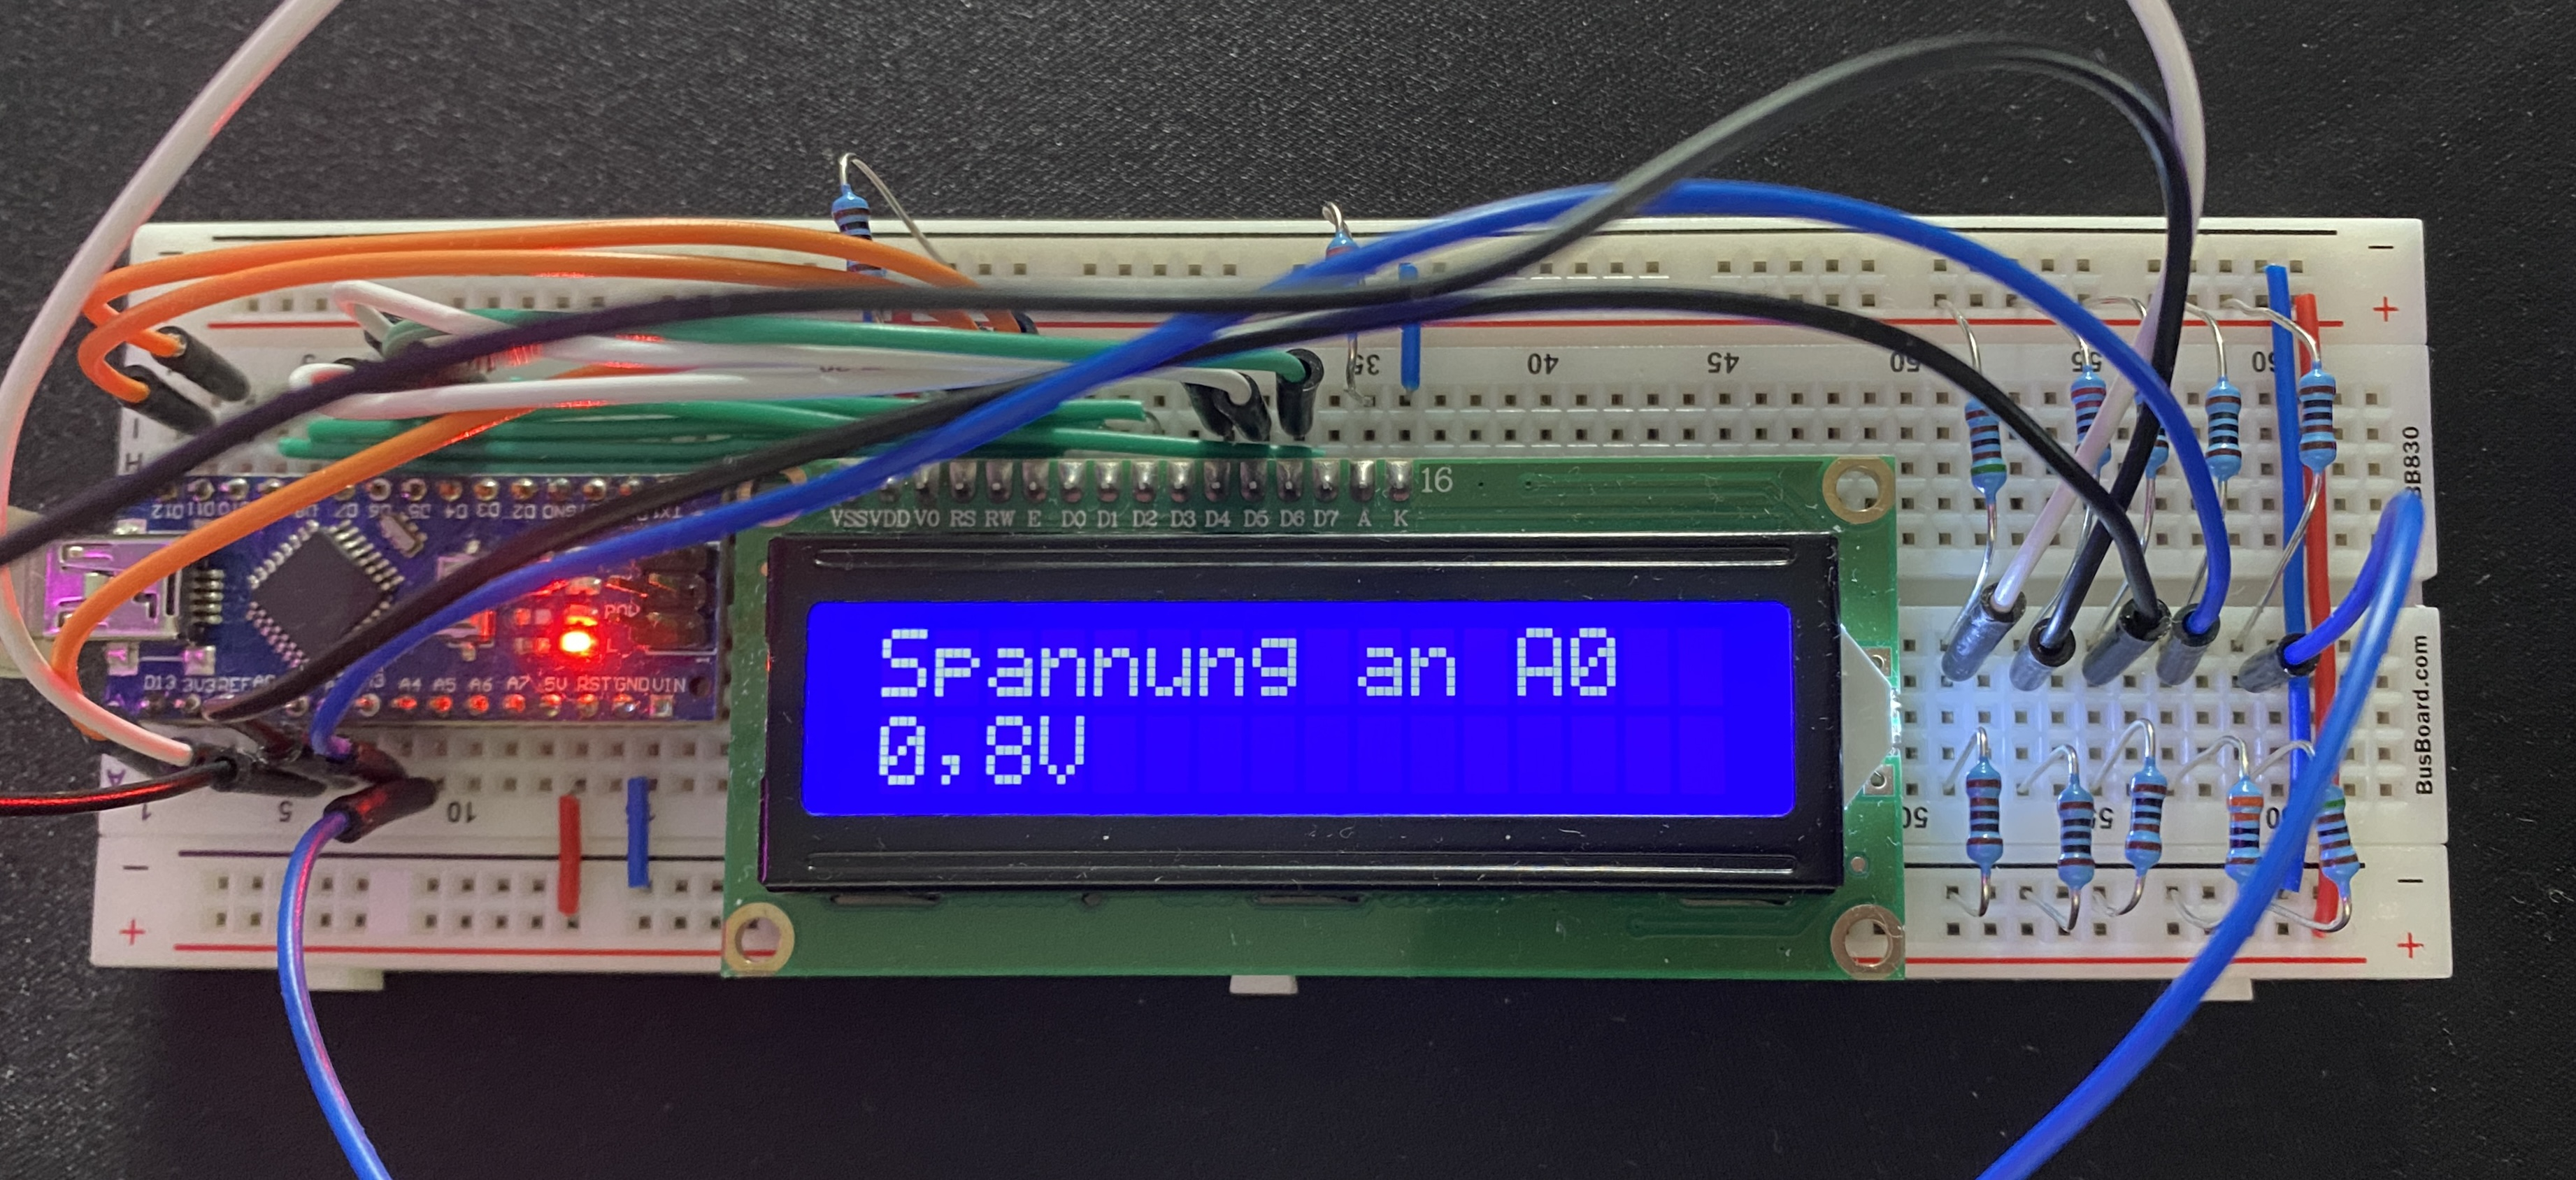
\includegraphics[width=0.8\linewidth]{schaltung.jpeg}
    \caption{Aufbau auf Breadboard}
\end{figure}

Die Betriebsspannung beträgt $U = \SI{5}{\volt}$.

Vorgegebene Spannungen die mit Widerstandskombinationen erstellt werden sollen:
\begin{align*}
    U_{A0} &\approx \SI{0.8}{\volt}\\
    U_{A1} &\approx \SI{1.6}{\volt}\\
    U_{A2} &\approx \SI{2.3}{\volt}\\
    U_{A3} &\approx \SI{3.7}{\volt}\\
    U_{A4} &\approx \SI{4.3}{\volt} 
\end{align*}

\begin{figure}
    \centering
    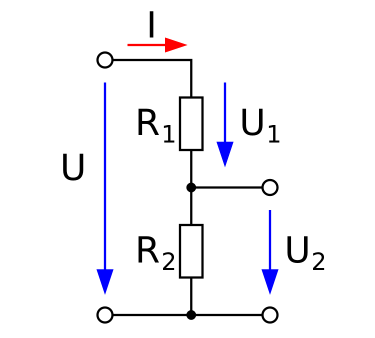
\includegraphics[width=0.4\linewidth]{spannungsteiler.png}
    \caption{Spannungsteiler (Quelle: wikipedia.org/wiki/Spannungsteiler)}
    \label{fig:spannungsteiler}
\end{figure}

\newpage
Diese Formel berechnet die Spannung an $R_2$ (vgl. Abbildung~\ref{fig:spannungsteiler}),
welche vom ATmega328P gelesen wird.
\begin{align*}
    U_2 &= U \cdot \frac{R_2}{R_1 + R_2}\\
\end{align*}

Zur Verfügung stehen diese Widerstände:
\begin{align*}
    R \in \{\SI{100}{\ohm}; \SI{220}{\ohm}; \SI{330}{\ohm}; \SI{1}{\kilo\ohm}; \SI{5.1}{\kilo\ohm}\}
\end{align*}

Die Toleranzen werden hier vernachlässigt, da die Widerstände eine geringe Toleranz von \SI{1}{\percent} haben 
und die Aufgabe nur ungefähre Spannungen vorgibt.
\begin{align*}
   &U_{A0} = \SI{5}{\volt} \cdot \frac{\SI{1}{\kilo\ohm}}{\SI{5.1}{\kilo\ohm} + \SI{1}{\kilo\ohm}} \approx \SI{0.82}{\volt}
   &&\text{für } R_1 = \SI{5.1}{\kilo\ohm}; R_2 = \SI{1}{\kilo\ohm}\\
   &U_{A1} = \SI{5}{\volt} \cdot \frac{\SI{100}{\ohm}}{\SI{220}{\ohm} + \SI{100}{\ohm}} \approx \SI{1.563}{\volt}
   &&\text{für } R_1 = \SI{220}{\ohm}; R_2 = \SI{100}{\ohm}\\
   &U_{A2} = \SI{5}{\volt} \cdot \frac{\SI{1}{\kilo\ohm}}{\SI{1}{\kilo\ohm} + \SI{1}{\kilo\ohm}} = \SI{2.5}{\volt}
   &&\text{für } R_1 = \SI{1}{\kilo\ohm}; R_2 = \SI{1}{\kilo\ohm}\\
   &U_{A3} = \SI{5}{\volt} \cdot \frac{\SI{330}{\ohm}}{\SI{100}{\ohm} + \SI{330}{\ohm}} \approx \SI{3.837}{\volt}
   &&\text{für } R_1 = \SI{100}{\ohm}; R_2 = \SI{330}{\ohm}\\
   &U_{A4} = \SI{5}{\volt} \cdot \frac{\SI{5.1}{\kilo\ohm}}{\SI{1}{\kilo\ohm} + \SI{5.1}{\kilo\ohm}} \approx \SI{4.18}{\volt}
   &&\text{für } R_1 = \SI{1}{\kilo\ohm}; R_2 = \SI{5.1}{\kilo\ohm}\\
\end{align*}

Um aus dem 10 Bit Messwert $x$ eine Spannung zu berechnen wird diese Formel verwendet:
\begin{align*}
    U_A &= U \cdot \frac{x}{1023}
    &&x \in [0; 1023]
\end{align*}

\clearpage
\lstinputlisting[language=c++]{../MessdatenLCD.ino}
\end{document}
